\documentclass[11pt]{article}
\usepackage[a4paper,margin=2cm]{geometry}
\usepackage{amsmath,amssymb,booktabs,xcolor,enumitem,colortbl,tabularx,array}
\newcolumntype{L}{>{\raggedright\arraybackslash}X}
\usepackage{tikz}
\usetikzlibrary{arrows.meta,positioning,calc}
\usepackage{pgfplots}
\pgfplotsset{compat=1.17}
\usepackage[hidelinks]{hyperref}
\setlist{nosep,leftmargin=1.4em}

\definecolor{arc}{HTML}{1F5FAD}
\definecolor{good}{HTML}{2E7D32}
\definecolor{bad}{HTML}{B3261E}
\definecolor{mid}{HTML}{D9730D}
\definecolor{soft}{HTML}{F2F2F2}
\newcommand{\gapgood}[1]{\textcolor{good}{\textbf{#1}}}
\newcommand{\gapmid}[1]{\textcolor{mid}{\textbf{#1}}}
\newcommand{\gapbad}[1]{\textcolor{bad}{\textbf{#1}}}
\tikzset{
  box/.style={draw,thick,rounded corners=3pt,align=center,minimum height=11mm,inner sep=4pt,font=\small},
  q/.style={box,fill=arc!10,draw=arc},
  c/.style={box,fill=soft},
  flow/.style={-{Stealth[length=2.6mm]},thick},
}

\title{\textbf{Quantum approaches to QOBLIB portfolio optimisation}\\[2pt]
\large Status report: exact ground truth, PCE quantum LNS, and quality vs.\ best known}
\date{22 November 2026 (updated: \S\ref{sec:qfocus} new formulations, \S\ref{sec:sparse} 200 and 400 assets)}
\author{}

\begin{document}
\sloppy
\maketitle
\vspace{-1cm}

%===========================================================================
\section*{Bottom line}
The score is QOBLIB's official objective, computed by the referee \texttt{PortfolioModel.score}; lower
is better. \emph{Gap} = (our score $-$ best known) / $|$best known$|$: \textbf{0\% matches QOBLIB,
negative beats it}. All 148 solution files written were re-scored from disk: all are feasible and
match the referee. All 127+ also pass QOBLIB's official Rust checker (\texttt{06-portfolio/check}),
which recomputes the objective in exact arithmetic and confirms every claimed value.

\begin{center}
\renewcommand{\arraystretch}{1.08}\footnotesize
\begin{tabularx}{\textwidth}{@{}>{\raggedright\arraybackslash}p{40mm}Lrr>{\raggedright\arraybackslash}p{30mm}@{}}
\toprule
instance ($B$, $\lambda$) & best result and method & score & gap & quantum used?\\
\midrule
\texttt{a010\_t10\_orig} (4, $10^{-4}$) & PCE quantum LNS from empty portfolio & $-69\,482$ & \gapgood{0.000\%} & \textbf{yes}: $\le$9 qubits\\
\texttt{a010\_t10\_orig} (4, $5\cdot10^{-4}$) & PCE quantum LNS from empty portfolio & $-27\,044$ & \gapgood{0.000\%} & \textbf{yes}: $\le$9 qubits\\
\texttt{a010\_t10\_orig} (4, $10^{-3}$) & PCE quantum LNS from empty portfolio & $-8\,397$ & \gapgood{0.000\%} & \textbf{yes}: $\le$9 qubits\\
\texttt{a010\_t10\_s02} (4, $10^{-4}$) & PCE quantum LNS from empty portfolio & $-53\,220$ & \gapmid{+0.066\%} & \textbf{yes}: $\le$9 qubits\\
all 64 \texttt{a010} instances & exact dynamic programming & $=$ BKV & \gapgood{0.000\%} & no: \emph{proves} all 64 optimal\\
\texttt{a050\_t10\_s00} (20, $10^{-2}$) & pool-DP + exact-DP LNS & $-17\,675$ & \gapgood{$-$43.2\%} & no (classical)\\
\texttt{a050\_t15\_orig} (20, $10^{-2}$) & pool-DP + exact-DP LNS & $-45\,031$ & \gapgood{$-$42.9\%} & no (classical)\\
\texttt{a050\_t15\_s02} (20, $10^{-2}$) & pool-DP + exact-DP LNS & $-41\,517$ & \gapgood{$-$2.2\%} & no (classical)\\
\texttt{a050\_t10\_s00} (20, $5\cdot10^{-4}$) & pool-DP + exact-DP LNS & $-234\,587$ & \gapgood{$-$0.14\%} & no (classical)\\
\texttt{a200\_t10\_orig} (50, $10^{-3}$) & pool-DP + LNS, 200 s & $-818\,362$ & first value & no (classical)\\
\texttt{a400\_t10\_orig} (100, $10^{-3}$) & pool-DP + LNS, 200 s, not converged & $-1\,896\,257$ & first value & no (classical)\\
\rowcolor{good!10}
\texttt{a050\_t10\_s00} (20, $10^{-4}$) & \textbf{PCE quantum LNS from empty portfolio} (new) & $\mathbf{-340\,222}$ & \gapgood{+4.31\%} & \textbf{yes}: $\le$9 qubits, 42 assets held\\
\texttt{a050\_t10\_s00} (20, $10^{-3}$) & PCE quantum LNS from empty portfolio (new) & $-157\,229$ & \gapmid{+18.1\%} & \textbf{yes}: $\le$9 qubits, 49 assets held\\
\texttt{a050\_t10\_s00} (20, $10^{-2}$) & best \emph{quantum}: PCE quantum LNS (stays empty; best non-empty $+37\,234$) & $-1\,000$ & \gapbad{+91.9\%} & yes: no useful result, \S\ref{sec:qfocus}\\
\rowcolor{good!10}
\texttt{a200\_t10\_orig} (50, $10^{-4}$) & \textbf{PCE quantum LNS from empty, block-sparse QUBO} (new) & $\mathbf{-794\,168}$ & first value & \textbf{yes}: $\le$9 qubits, 154 assets held\\
\rowcolor{good!10}
\texttt{a400\_t10\_orig} (100, $10^{-4}$) & \textbf{PCE quantum LNS from empty, block-sparse QUBO} (new) & $\mathbf{-1\,397\,396}$ & first value & \textbf{yes}: $\le$10 qubits, 313 assets held\\
\texttt{a200\_t10\_orig} (50, $10^{-3}$) & PCE quantum LNS from empty (new); classical $-818\,362$ & $-469\,837$ & 43\% worse & yes: $\le$9 qubits\\
\bottomrule
\end{tabularx}
\end{center}

\noindent\textbf{In one sentence:} a quantum sub-solver (Divi PCE, at most 9 qubits, on a 630-variable
QUBO) reaches the \emph{proven} optimum on three leaderboard instances, starting from an empty
portfolio without any classical local search. On \textbf{50 assets} the same method, again from an
empty portfolio, gets within \textbf{+4.3\%} of the best known value at $\lambda=10^{-4}$, holding
20 units on 42 assets every day. At the risk-dominated $\lambda=10^{-2}$ no quantum formulation has
worked yet (\S\ref{sec:qfocus}). With a block-sparse QUBO (\S\ref{sec:sparse}) the method also runs on
\textbf{200 and 400 assets} (12\,100 and 24\,110 variables) and gives the first quantum values for
\texttt{a200} and \texttt{a400} at $\lambda=10^{-4}$, where QOBLIB publishes nothing. The four best-known
values we beat on 50-asset instances were beaten by classical search.

%===========================================================================
\section{The problem in one paragraph}
For $T$ days and $n$ stocks, decide how many units to hold long and short (0--3 each). The objective
is $\lambda\cdot$risk $-$ returns $+$ transaction costs $-$ interest on idle cash $+$ short fees $+$
liquidation costs. Two rules hold on every day: the net position lies in $[C-15,\,C]$ with $C=10$,
and at most $B$ units are open. QOBLIB's model uses one bit per (asset, unit copy, direction, day)
plus slack registers: 710 bits for $10\times10$, about 3\,500 for $50\times10$.

\paragraph{Four facts read off the referee code} (they drive everything below).
\begin{itemize}
\item \textbf{Interest is linear:} it equals $-10\,(C-\text{net})$ per day, so no cash slack bits are needed.
\item \textbf{Long and short together is dominated:} same net position, extra fees and
  $|\Delta L|+|\Delta S|\ge|\Delta v|$. So the state per (day, asset) is $v=L-S\in\{-3,\dots,3\}$.
\item \textbf{With $B=4$ the capital rule cannot bind} (net $\in[-4,4]\subset[-5,10]$); only the budget matters.
\item The last day is always empty (no return, liquidation cost, free move into it).
\end{itemize}

%===========================================================================
\section{Ground truth: exact DP proves all 64 ten-asset BKVs optimal}
Days are coupled only by the rebalancing cost $\sum_i \mathrm{tc}_{t,i}\,|v_{t,i}-v_{t-1,i}|$. With
the reduced state, a day has only 8\,341 feasible vectors ($\sum_i|v_i|\le4$, $n=10$). A dynamic
program over days (numba min-plus step with pruning) is therefore exact and takes about 2\,s per instance.
\begin{itemize}
\item Validated against the referee's \texttt{brute\_force} (3 assets, $B=2,3,4$) and the 10 BKVs that
  QOBLIB labels \emph{optimal}.
\item \textbf{All 64 \texttt{a010} instances: DP optimum $=$ BKV.} 54 of them are labelled only
  ``best known''; they are now proven optimal. Nothing can be beaten at 10 assets.
\item This gives the quantum runs an exact target: the gap of every quantum result is a true optimality gap.
\end{itemize}

%===========================================================================
\section{The quantum pipeline: PCE quantum large-neighbourhood search}
\begin{center}
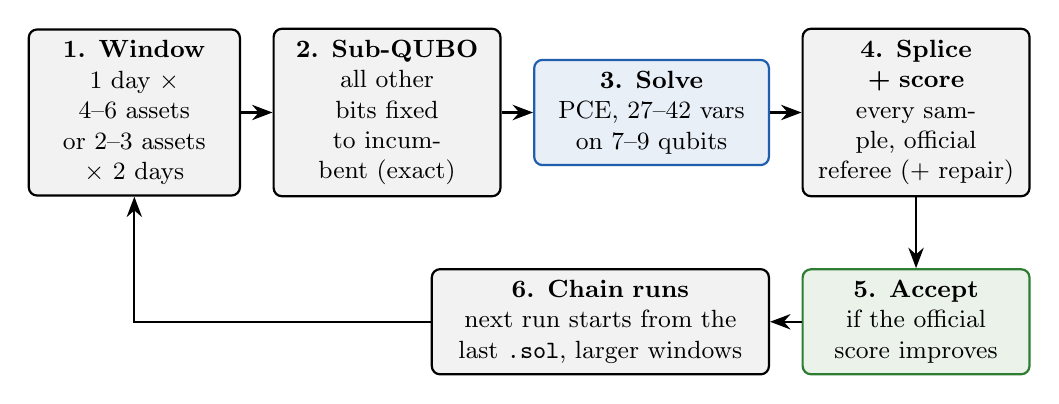
\begin{tikzpicture}[node distance=4mm and 4mm]
  \node[c,text width=24mm] (win) {\textbf{1. Window}\\1 day $\times$ 4--6 assets\\or 2--3 assets $\times$ 2 days};
  \node[c,right=of win,text width=26mm] (sub) {\textbf{2. Sub-QUBO}\\all other bits fixed\\to incumbent (exact)};
  \node[q,right=of sub,text width=27mm] (pce) {\textbf{3. Solve}\\PCE, 27--42 vars\\on 7--9 qubits};
  \node[c,right=of pce,text width=26mm] (spl) {\textbf{4. Splice + score}\\every sample, official\\referee (+ repair)};
  \node[box,fill=good!10,draw=good,below=9mm of spl,text width=26mm] (acc) {\textbf{5. Accept}\\if the official\\score improves};
  \node[c,left=of acc,text width=40mm] (chain) {\textbf{6. Chain runs}\\next run starts from the last \texttt{.sol}, larger windows};
  \draw[flow] (win)--(sub); \draw[flow] (sub)--(pce); \draw[flow] (pce)--(spl);
  \draw[flow] (spl)--(acc); \draw[flow] (acc)--(chain);
  \draw[flow] (chain.west) -| (win.south);
\end{tikzpicture}
\end{center}
\noindent\textcolor{arc}{\textbf{Blue}} = quantum step. No classical optimiser or local search is
inside the loop. The only classical parts are the referee's greedy repair of infeasible splices and the
accept-if-better rule.

\paragraph{Key ingredients.}
\begin{itemize}
\item \textbf{Compact QUBO} (\texttt{CompactQUBO}): the official unary copies, interest folded into the objective, a
  3-bit budget slack and no cash register: \textbf{630 variables} (official: 710). Its energy equals the referee's
  objective on every tested portfolio. For $B>5$ the 4-bit cash register is added back (3\,090 vars for
  \texttt{a050\_t10}).
\item \textbf{PCE} (Divi, \texttt{PolyEncoding}, 3 layers, \texttt{SoftObjective}($\alpha{=}2$),
  Monte Carlo optimiser $40\times8$, local Maestro): one window of 27--42 variables fits on 7--9 qubits and
  takes about 1\,s.
\item \textbf{Penalty weight} 5000 inside windows. The service recommended $\lambda\approx0.1$ for an
  empty-incumbent window, where the budget cannot bind; next to held positions it does bind.
\end{itemize}

\subsection{Results on \texttt{po\_a010\_t10\_orig}, $B=4$ (DP-proven optima)}
\begin{center}\small
\begin{tabularx}{\textwidth}{@{}Lrrrrr@{}}
\toprule
$\lambda$ (runs chained) & PCE-QLNS result & optimum & gap & circuits & time\\
\midrule
\rowcolor{good!10}
$10^{-4}$ (2 runs) & $\mathbf{-69\,482}$ & $-69\,482$ & \gapgood{0.000\%} & 0.22\,M & 19 min\\
\rowcolor{good!10}
$5\cdot10^{-4}$ (2 runs) & $\mathbf{-27\,044}$ & $-27\,044$ & \gapgood{0.000\%} & 0.29\,M & 21 min\\
\rowcolor{good!10}
$10^{-3}$ (3 runs) & $\mathbf{-8\,397}$ & $-8\,397$ & \gapgood{0.000\%} & 0.91\,M & 31 min\\
\texttt{a010\_t10\_s02}, $10^{-4}$ (2 runs) & $-53\,220$ & $-53\,255$ & \gapmid{+0.066\%} & 0.73\,M & 18 min\\
\midrule
\multicolumn{6}{@{}l}{\emph{References on the same instance ($\lambda=10^{-4}$ unless stated)}}\\
notebook 01, partitioned QAOA + local search (3 seeds) & $-69\,169$ & & +0.45\% & 0.1\,M & 2 min\\
notebook starter SA + LS, $\lambda=5\cdot10^{-4}$ / $10^{-3}$ & $-26\,548$ / $-3\,703$ & & +1.8\% / +56\% & -- & --\\
our route B: partitioned QAOA, stitched + repair & $-3\,484$ & & \gapbad{+95\%} & 31\,k & 79 s\\
\quad + referee local search & $-54\,923$ & & \gapbad{+21\%} & & \\
QLNS with warm-started QAOA (15--18 qubits) from route B & $-68\,249$ & & \gapmid{+1.8\%} & 30\,k & 20 min\\
\bottomrule
\end{tabularx}
\end{center}

\begin{center}
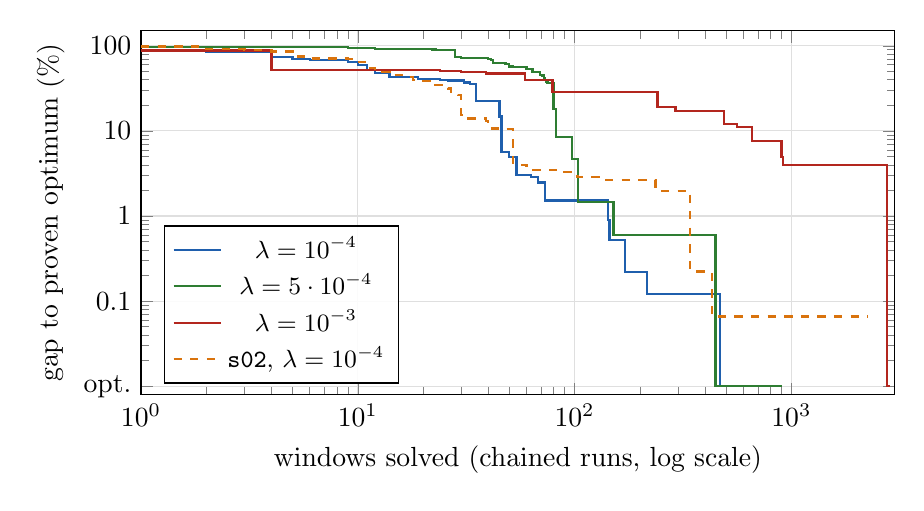
\begin{tikzpicture}
\begin{axis}[width=0.92\textwidth,height=6.2cm,ymode=log,xmode=log,
  xlabel={windows solved (chained runs, log scale)},ylabel={gap to proven optimum (\%)},
  ymin=0.008,ymax=150,xmin=1,xmax=3000,grid=major,grid style={gray!25},
  legend pos=south west,legend style={font=\small,fill=white,fill opacity=0.9,text opacity=1},
  ytick={0.01,0.1,1,10,100},yticklabels={opt.,0.1,1,10,100}]
\addplot[thick,arc] coordinates {(1,97.211) (2,97.211) (2,85.519) (3,85.519) (3,84.697) (4,84.697) (4,73.366) (5,73.366) (5,70.199) (6,70.199) (6,68.026) (7,68.026) (7,67.653) (9,67.653) (9,64.899) (10,64.899) (10,58.948) (11,58.948) (11,52.120) (12,52.120) (12,47.812) (14,47.812) (14,42.899) (19,42.899) (19,40.957) (24,40.957) (24,40.043) (25,40.043) (25,39.987) (26,39.987) (26,39.197) (31,39.197) (31,37.113) (33,37.113) (33,35.943) (35,35.943) (35,22.629) (36,22.629) (36,22.590) (41,22.590) (41,22.537) (45,22.537) (45,14.775) (46,14.775) (46,5.623) (50,5.623) (50,4.944) (54,4.944) (54,3.035) (63,3.035) (63,2.901) (68,2.901) (68,2.475) (73,2.475) (73,1.523) (142,1.523) (142,0.889) (145,0.889) (145,0.528) (171,0.528) (171,0.219) (216,0.219) (216,0.122) (467,0.122) (467,0.010) (701,0.010)}; \addlegendentry{$\lambda=10^{-4}$}
\addplot[thick,good] coordinates {(1,96.302) (9,96.302) (9,94.716) (12,94.716) (12,91.299) (16,91.299) (16,91.089) (22,91.089) (22,90.671) (23,90.671) (23,89.084) (28,89.084) (28,73.931) (30,73.931) (30,71.635) (33,71.635) (33,71.491) (40,71.491) (40,69.982) (41,69.982) (41,67.664) (42,67.664) (42,63.371) (44,63.371) (44,62.676) (48,62.676) (48,61.034) (50,61.034) (50,57.155) (52,57.155) (52,56.245) (60,56.245) (60,53.923) (64,53.923) (64,49.183) (66,49.183) (66,48.924) (69,48.924) (69,45.145) (71,45.145) (71,44.838) (72,44.838) (72,42.290) (73,42.290) (73,39.613) (74,39.613) (74,37.864) (75,37.864) (75,36.577) (80,36.577) (80,17.934) (82,17.934) (82,8.434) (97,8.434) (97,4.648) (104,4.648) (104,1.475) (151,1.475) (151,0.599) (447,0.599) (447,0.010) (901,0.010)}; \addlegendentry{$\lambda=5\cdot10^{-4}$}
\addplot[thick,bad] coordinates {(1,88.091) (4,88.091) (4,51.637) (18,51.637) (18,51.566) (24,51.566) (24,50.911) (30,50.911) (30,48.887) (39,48.887) (39,47.410) (59,47.410) (59,39.407) (79,39.407) (79,28.427) (241,28.427) (241,19.007) (292,19.007) (292,17.089) (490,17.089) (490,11.957) (563,11.957) (563,11.063) (657,11.063) (657,7.598) (901,7.598) (901,4.966) (918,4.966) (918,3.966) (2752,3.966) (2752,0.010) (2838,0.010)}; \addlegendentry{$\lambda=10^{-3}$}
\addplot[thick,mid,dashed] coordinates {(1,98.122) (2,98.122) (2,91.646) (3,91.646) (3,88.705) (4,88.705) (4,85.630) (5,85.630) (5,74.992) (6,74.992) (6,70.981) (7,70.981) (7,70.957) (9,70.957) (9,70.061) (10,70.061) (10,64.661) (11,64.661) (11,55.163) (12,55.163) (12,51.796) (13,51.796) (13,49.342) (14,49.342) (14,45.235) (16,45.235) (16,45.192) (17,45.192) (17,43.395) (18,43.395) (18,39.996) (20,39.996) (20,38.849) (22,38.849) (22,34.288) (26,34.288) (26,31.443) (27,31.443) (27,27.327) (29,27.327) (29,26.345) (30,26.345) (30,15.473) (31,15.473) (31,14.224) (32,14.224) (32,13.955) (39,13.955) (39,13.034) (40,13.034) (40,10.694) (46,10.694) (46,10.448) (52,10.448) (52,4.187) (55,4.187) (55,4.015) (60,4.015) (60,3.853) (63,3.853) (63,3.489) (88,3.489) (88,3.271) (99,3.271) (99,2.927) (103,2.927) (103,2.854) (140,2.854) (140,2.640) (236,2.640) (236,1.987) (342,1.987) (342,0.223) (429,0.223) (429,0.066) (2260,0.066)}; \addlegendentry{\texttt{s02}, $\lambda=10^{-4}$}
\end{axis}
\end{tikzpicture}
\end{center}
\noindent\textbf{Reading:} every chain starts from the empty portfolio (gap 88--98\%). It gets within
1\% after a few hundred windows, and the larger windows of the follow-up runs close the last step to
the optimum. The bottom of the axis (``opt.'') means the proven optimum was reached.

\paragraph{PCE versus QAOA as the window solver.} QAOA (X mixer, 4 layers, warm-started from
\texttt{characterize\_and\_validate} angles, as in notebook~00) is a good sampler. The exact window
optimum was among its 64 most likely bitstrings in \textbf{145 of 200} windows (73\%). But a
15--18-qubit window costs 2--18\,s and holds only 2 assets, against about 1\,s for a 4--6-asset PCE
window on 7--9 qubits. Larger windows escape local optima, so at equal wall time PCE wins
($-69\,397$ against $-68\,249$ after 20 minutes).


\subsection{All quantum results, including the weak ones}\label{sec:allq}
Every quantum configuration we ran, with its best official score. The gap is measured against QOBLIB's
BKV, which is the proven optimum on every \texttt{a010} instance. ``Our best'' is the best score from any
method, classical included. Runs marked $^\dagger$ were stopped early and their score comes from the
log; no \texttt{.sol} was written.
\begin{center}\small
\renewcommand{\arraystretch}{1.15}
\begin{tabularx}{\textwidth}{@{}>{\raggedright\arraybackslash}p{30mm}Lrrrr@{}}
\toprule
instance, $\lambda$ & quantum configuration & qubits & circuits & best score & gap vs BKV\\
\midrule
\texttt{a010\_t10\_orig}, $10^{-4}$ & \textbf{PCE-QLNS, 2 chained runs from empty} & $\le$9 & 0.22\,M & $\mathbf{-69\,482}$ & \gapgood{0.000\%}\\
\footnotesize BKV $-69\,482$ (opt.) & PCE-QLNS, single run from empty & 8 & 96\,k & $-69\,397$ & \gapmid{+0.12\%}\\
 & PCE-QLNS, single run, larger windows & 9 & 0.13\,M & $-68\,785$ & \gapmid{+1.00\%}\\
 & QAOA-QLNS, warm start, from route-B start & $\le$18 & 30\,k & $-68\,249$ & \gapmid{+1.77\%}\\
 & QAOA-QLNS, warm start, from empty$^\dagger$ (59 windows) & $\le$18 & -- & $-54\,272$ & \gapbad{+21.9\%}\\
 & partitioned QAOA + repair + referee local search & 12 & 31\,k & $-54\,923$ & \gapbad{+21.0\%}\\
 & partitioned QAOA + repair only & 12 & 31\,k & $-3\,484$ & \gapbad{+95.0\%}\\
\midrule
\texttt{a010\_t10\_orig}, $5\cdot10^{-4}$ & \textbf{PCE-QLNS, 2 chained runs from empty} & $\le$9 & 0.29\,M & $\mathbf{-27\,044}$ & \gapgood{0.000\%}\\
\footnotesize BKV $-27\,044$ (opt.) & PCE-QLNS, single run from empty & 8 & 0.13\,M & $-26\,882$ & \gapmid{+0.60\%}\\
\midrule
\texttt{a010\_t10\_orig}, $10^{-3}$ & \textbf{PCE-QLNS, 3 chained runs from empty} & $\le$9 & 0.91\,M & $\mathbf{-8\,397}$ & \gapgood{0.000\%}\\
\footnotesize BKV $-8\,397$ (opt.) & after 2 chained runs & $\le$9 & 0.29\,M & $-7\,759$ & \gapmid{+7.6\%}\\
 & PCE-QLNS, single run from empty & 8 & 0.13\,M & $-6\,962$ & \gapbad{+17.1\%}\\
\midrule
\texttt{a010\_t10\_s02}, $10^{-4}$ & \textbf{PCE-QLNS, 2 chained runs from empty} & $\le$9 & 0.73\,M & $\mathbf{-53\,220}$ & \gapmid{+0.066\%}\\
\footnotesize BKV $-53\,255$ (opt.) & PCE-QLNS, single run & 8 & 0.13\,M & $-53\,136$ & \gapmid{+0.22\%}\\
\midrule
\rowcolor{good!10}
\texttt{a050\_t10\_s00}, $10^{-4}$ & \textbf{PCE-QLNS from empty}, 1 run, 2\,805 windows (new) & $\le$9 & 0.90\,M & $\mathbf{-340\,222}$ & \gapgood{+4.31\%}\\
\footnotesize BKV $-355\,530$ & & & & & \\
\midrule
\texttt{a050\_t10\_s00}, $10^{-3}$ & \textbf{PCE-QLNS from empty}, 1 run, 2\,933 windows (new) & $\le$9 & 0.94\,M & $\mathbf{-157\,229}$ & \gapmid{+18.1\%}\\
\footnotesize BKV $-191\,879$ & & & & & \\
\midrule
\texttt{a050\_t10\_s00}, $10^{-2}$ & \textbf{PCE-QLNS from empty}$^\dagger$, 3 runs, 359 windows & $\le$9 & -- & $\mathbf{-1\,000}$ & \gapbad{+91.9\%}\\
\footnotesize BKV $-12\,340$; ours (classical) $-17\,675$ & PCE-QLNS from an over-full start: rounded relaxation (new) & $\le$9 & 0.85\,M & $+37\,234$ & \gapbad{+402\%}\\
 & PCE-QLNS from an over-full start: our $\lambda=10^{-3}$ portfolio (new) & $\le$9 & 0.85\,M & $+69\,194$ & \gapbad{+661\%}\\
 & Q-MOVES, PCE, 24 or 60 moves, from the same start$^\dagger$ (new) & 7--11 & -- & no change & --\\
 & Q-MOVES, QAOA, 18 moves, Qoro \texttt{qoro\_cpu} cloud$^\dagger$ (new) & 18 & -- & no change & --\\
 & PCE-QLNS from the classical $-17\,675$ & $\le$9 & 0.19\,M & no change & (classical)\\
\midrule
\texttt{a050\_t10\_orig}, $10^{-2}$ & XY-exchange QAOA from the classical $-34\,520$ (new, smoke test) & $\le$11 & 324 & no change & \footnotesize (classical +6.97\%)\\
\bottomrule
\end{tabularx}
\end{center}
\noindent Circuits ran on the local Maestro simulator, except the 18-qubit Q-MOVES QAOA (Qoro
\texttt{qoro\_cpu} cloud) and one \texttt{characterize\_and\_validate} job for the QAOA warm start.
The $-1\,000$ on \texttt{a050} at $\lambda=10^{-2}$ is the empty portfolio: no window changed it. The
over-full starts descend steadily but are still far from good after 30 minutes.

%===========================================================================
\section{Fifty assets and beyond}\label{sec:a050}
\paragraph{Classical (sub-agent, \texttt{lns.py}).} At high $\lambda$ the good portfolios hold about
15--37 assets at $\pm1$ unit with the budget used up. Single-unit moves never reach them: one unit on
its own is too risky, so SA and local search stay at the empty portfolio. The method that works:
\begin{enumerate}
\item build a candidate pool for each day: convex relaxation rounded at many scales, pair-move descent, ILS, SA;
\item run an exact DP that picks one pool vector per day, with true transaction costs;
\item run an LNS that re-optimises $k\le4$ assets exactly over all days.
\end{enumerate}
Result: \textbf{4 BKVs beaten} (table above). QOBLIB's official Rust checker confirms all four
as feasible, with exactly the objective values shown. On \texttt{a050\_t10}, 13 of 29 instances run match the
BKV exactly, and the $\lambda=10^{-3}\ldots10^{-6}$ instances are within 0--1.7\%. Still behind:
$\lambda=10^{-2}$ on \texttt{orig} (+7.0\%), \texttt{s02} (+7.8\%) and \texttt{s01} (+55\%, stuck at the empty portfolio).

\paragraph{Quantum on 50 assets.} PCE-QLNS scales technically: conditional sub-QUBOs are taken from a dense
$3\,090\times3\,090$ matrix in milliseconds. \textbf{How well it works depends on $\lambda$:}
\begin{itemize}
\item $\lambda=10^{-4}$, from empty: $\mathbf{-340\,222}$, \gapgood{+4.31\%}. The portfolio holds 20 units
  every day on 42 different assets, so it is far from trivial. It took 0.9\,M circuits on at most 9 qubits
  in 30 minutes on a laptop.
\item $\lambda=10^{-3}$, from empty: $-157\,229$, \gapmid{+18.1\%}, still improving when the 30-minute
  limit hit.
\item $\lambda=10^{-2}$, from empty: it stays at $-1000$ (the empty portfolio) with random,
  correlation-guided and multi-day ``hedge'' windows. A small window only sees moves that cost more than
  they gain. From the classical $-17\,675$, 600 windows found nothing better.
\end{itemize}

%===========================================================================
\section{Quantum focus: new formulations for the hard case}\label{sec:qfocus}
Goal: a quantum result within $+10\%$ of the best known value at 50 assets, which is not the empty
portfolio. Code is in \texttt{portfolio\_QIcing/quantum\_focus/}.

\paragraph{Why $\lambda=10^{-2}$ is hard (diagnosis).} The day-$t$ risk matrix has a few huge
eigenvalues: $674\,714$, $256\,935$, $161\,992$, \dots, against a median of $1\,539$. These are
market-wide factors. The best known day portfolios have \textbf{zero exposure to the top 5 factors}.
In any bit-level QUBO, once normalised for PCE or QAOA, these factor terms swamp the small differences
between good portfolios. Adding units from an empty portfolio is always uphill, and so is any small
change to the portfolio.

\begin{center}\small
\renewcommand{\arraystretch}{1.18}
\begin{tabularx}{\textwidth}{@{}>{\raggedright\arraybackslash}p{30mm}L>{\raggedright\arraybackslash}p{44mm}@{}}
\toprule
formulation & idea & outcome\\
\midrule
\textbf{Lower $\lambda$, PCE windows from empty} & same pipeline as \S3; the risk term is 10--100$\times$ smaller & \textcolor{good}{\textbf{works}}: +4.31\% at $10^{-4}$, +18.1\% at $10^{-3}$\\
Q-ROUND: quantum rounding & classical convex relaxation of each day, then a QUBO over the rounding bits $v_i=\lfloor w_i\rfloor+b_i$ (exact: $|v|$ stays linear). PCE samples the roundings, and an exact DP chains the days & \textcolor{bad}{fails}: even the \emph{optimal} rounding costs $+8\,293$ against $-6\,900$ for the best day. Good portfolios are not near the relaxation\\
Hedge-pair basis & variables are long-$a$/short-$b$ pairs (net 0, so the capital rule holds by construction) & \textcolor{bad}{fails}: no single pair is profitable; the profit comes only from baskets of about 20 units\\
\textbf{XY-exchange QAOA} (2-exchange analogue) & the circuit starts \emph{in} the incumbent (\texttt{CustomPerQubitState}); an XY mixer on same-day edges moves units between assets, so the unit count is conserved and the budget holds by construction & verified: the unit count is conserved in \textbf{100\%} of samples. No gain from the classical optimum, which is already exact for every 4-asset neighbourhood\\
\textbf{Q-MOVES}: move-selection QUBO & binary $y_m$ = apply move $m$ (transfer, flip, shift, extend/shrink, drop, add-hedge). The energy $E(x{+}D^\top y)=E(x)+y\cdot D(h{+}Sx)+\tfrac12 y^\top DSD^\top y$ is exact & exact: \textbf{0 mismatches} in 880 checks. SA on it improves steadily. PCE samples are near random (no gain), and QAOA on \texttt{qoro\_cpu} takes about 2\,min per round with no gain\\
Over-full starts & start from a full but too risky portfolio (rounded relaxation, or our $\lambda=10^{-3}$ portfolio), so that moves go downhill & descends from $+640\,600$ to $+37\,234$, still far from the target\\
$\lambda$-homotopy & quantum windows follow the optimum from $\lambda=10^{-3}$ through 1.5--7.5$\cdot10^{-3}$ to $10^{-2}$ & \textcolor{bad}{fails}: the score turns positive by $7\cdot10^{-3}$ ($+5\,547$, $+22\,464$); both chains were stopped before the last step\\
\bottomrule
\end{tabularx}
\end{center}

\noindent\textbf{Reading:} the move and exchange formulations are correct and exact. What limits them
is the samplers: at 18--60 variables, PCE and QAOA as configured here return nearly uniform samples on
these QUBOs, while SA on the same QUBO improves the portfolio. The quantum result that meets the target
is the plain PCE window method at moderate risk ($\lambda=10^{-4}$).

%===========================================================================
\section{Two hundred and four hundred assets: block-sparse QUBO}\label{sec:sparse}
The dense compact QUBO needs $n_\text{vars}^2$ entries: 2.3\,GB for \texttt{a200} and 9\,GB for
\texttt{a400}, on a 9\,GB machine. But every coupling lies \emph{inside one day} (risk, budget and capital
penalties) or links \emph{the same unit bit on adjacent days} (rebalancing). So \texttt{sparse/block\_qubo.py}
stores one dense float32 block per day plus one weight per bit for the adjacent-day link, and cuts
window sub-QUBOs out of the blocks.

\begin{center}\small
\begin{tabularx}{\textwidth}{@{}Lrrrrr@{}}
\toprule
instance & QUBO variables & block memory & dense equivalent & build & window sub-QUBO\\
\midrule
\texttt{a200\_t10} & 12\,100 & \textbf{56\,MB} & 2.3\,GB & 0.4\,s & 5\,ms\\
\texttt{a400\_t10} & 24\,110 & \textbf{222\,MB} & 9\,GB & 2\,s & 1.4\,ms\\
\bottomrule
\end{tabularx}
\end{center}
\noindent Validated on \texttt{a050} against the dense version: full energies are identical, window
energy differences show zero error over 100 checks, and on feasible portfolios the energy equals the
official referee (20 of 20). The window solver is unchanged, PCE on at most 9--10 qubits on the local
Maestro simulator. Window size does not grow with the instance, so the circuits need no cloud.

\begin{center}\small
\begin{tabularx}{\textwidth}{@{}Lrrrrr@{}}
\toprule
instance, $\lambda$ (60 min, from empty) & result & assets held & units/day & windows & circuits\\
\midrule
\rowcolor{good!10}
\texttt{a200\_t10\_orig}, $10^{-4}$ & $\mathbf{-794\,168}$ & 154 & 50 of 50 & 9\,424 & 3.0\,M\\
\rowcolor{good!10}
\texttt{a400\_t10\_orig}, $10^{-4}$ & $\mathbf{-1\,397\,396}$ & 313 & 100 of 100 & 6\,866 & 2.2\,M\\
\texttt{a200\_t10\_orig}, $10^{-3}$ & $-469\,837$ & 160 & 49--50 of 50 & 9\,479 & 3.0\,M\\
\quad classical reference (pool-DP + LNS, 200\,s) & $-818\,362$ & & & & \\
\bottomrule
\end{tabularx}
\end{center}
\noindent\textbf{Reading:} QOBLIB has no published values for any \texttt{a200} or \texttt{a400}
instance, so the two $\lambda=10^{-4}$ results are first values, and they come from quantum windows
alone. They are not converged: all runs were still improving at the 60-minute cut, and \texttt{a400}
saw only 6\,866 windows for 400 assets. Where a comparison exists, at \texttt{a200} $\lambda=10^{-3}$,
the quantum run is 43\% short of our classical result, so quality at this scale is unproven. Both
$\lambda=10^{-4}$ runs fill the budget on every trading day and spread it over 154 and 313 assets.

%===========================================================================
\section{Main lessons}
\begin{enumerate}
\item \textbf{Know the true optimum first.} The reduced-state DP turned 54 ``best known'' values into
  proven optima in two minutes. It showed that nothing can be beaten at 10 assets and gave the quantum
  runs an exact target.
\item \textbf{Shrink the QUBO using the referee's structure.} Linear interest and the inactive capital
  rule remove all cash slack bits; the dominance argument halves the effective search space.
\item \textbf{Small windows, many of them.} Full-QUBO partitioning cuts through the budget
  constraints, and the stitched output is +95\% off. Exact conditional windows keep every
  constraint and solve every sub-problem exactly as posed.
\item \textbf{PCE fits windows better than QAOA.} It packs 3--5$\times$ more variables per qubit,
  so windows are larger and solved faster.
\item \textbf{At 50 assets quantum windows can build, up to moderate risk.} From an empty portfolio,
  PCE windows reach +4.3\% at $\lambda=10^{-4}$ and +18\% at $10^{-3}$. At $\lambda=10^{-2}$ the
  optima are factor-neutral baskets, and a constructor (the per-day pool plus DP) is still needed.
\item \textbf{The landscape, not the formulation, is the obstacle at high risk.} A few market factors
  dominate the risk matrix by about 400$\times$. Exact move and exchange QUBOs are easy to write, but
  PCE and QAOA as configured here do not concentrate on them. Better-conditioned encodings, with the
  dominant factors projected out, are the next lever.
\item \textbf{Memory, not qubits, limits scale.} Windows stay at 9--10 qubits at any size. What breaks
  at 200+ assets is the classical QUBO storage, and the day-block structure fixes it (56\,MB and 222\,MB).
\end{enumerate}

\section{Next steps}
\begin{enumerate}
\item Chain more PCE runs on \texttt{a050} at $\lambda=10^{-4}$ and $10^{-3}$. The \texttt{a010} chains
  closed their last gap this way, and both 30-minute runs were still improving.
\item Run \texttt{a200}/\texttt{a400} longer, or chain runs as on \texttt{a010}, and add the remaining $\lambda$ values
  and seeds. The runs were still improving. For \texttt{a400}, batch many disjoint windows per
  \texttt{qoro\_cpu} job to raise throughput.
\item Make the hard case quantum-friendly: subtract the top risk factors and enforce zero exposure to them
  as constraints (XY or Dicke subspaces), so that the QUBO's scale reflects returns and residual risk.
\item Plug PCE into the classical LNS sub-solver hook (\texttt{lns.lns(..., solve\_sub=f)}). Still open.
\item The quantum per-day candidate pool was tried (Q-ROUND) and does not work in its rounding form.
  Cloud QAOA at 18 qubits works, but at about 2\,min per round it is too slow for LNS loops; batch
  many windows per cloud job instead.
\end{enumerate}

\vfill\noindent\footnotesize
Code in \texttt{portfolio\_QIcing/}: \texttt{pf\_core.py} (BKV table, exact DP, solution bookkeeping),
\texttt{pf\_quantum.py} (compact QUBO, dense sub-QUBOs, windows), \texttt{run\_qlns.py} (quantum LNS),
\texttt{run\_partitioned.py} (notebook route B), \texttt{lns.py}/\texttt{run\_lns.py} (classical, large instances),
\texttt{verify\_solutions.py} (re-scores every \texttt{.sol} into \texttt{best\_solutions.md}), \texttt{quantum\_focus/} (Q-ROUND, Q-EXCHANGE, Q-MOVES, homotopy), \texttt{sparse/} (block-sparse QUBO, \texttt{a200}/\texttt{a400} runner). Every run is
in \texttt{results.csv}, the solutions are in \texttt{solutions/}, and the notes are in \texttt{NOTES.md} and \texttt{NOTES\_lns.md}.
\end{document}
